\section{Messung der S-Parameter im NA-Modus}
Die PCB mit dem Coupled-Line-Filter wird mit dem Fieldfox an beiden Ausgängen angeschlossen, 
    woraufhin die S-Parameter dessen im Network-Analyzer-Modus vermessen werden. Folgende Leistungsspektren kommen zustande:
    \begin{figure}[H]
        
        \begin{minipage}{0.45\textwidth}
            \centering
            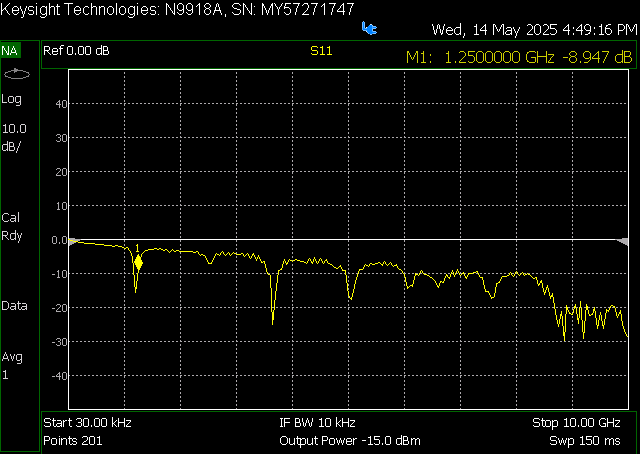
\includegraphics[width=\linewidth]{Pictures/S11neuCooleGrupp.png}
            \caption*{S11}
        \end{minipage}
        \hfill
        \begin{minipage}{0.45\textwidth}
            \centering
            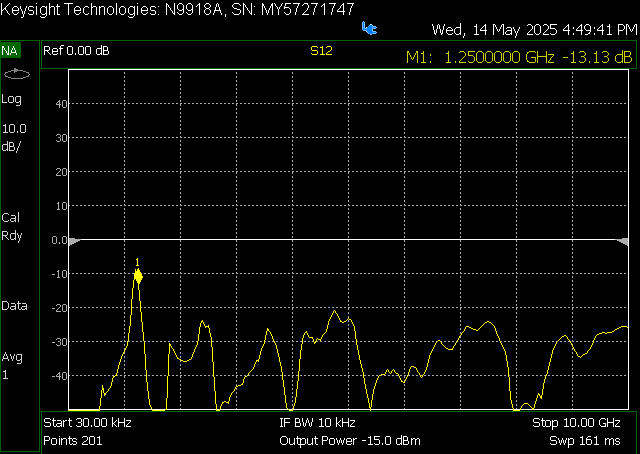
\includegraphics[width=\linewidth]{Pictures/S12neuCooleGrupp.png}
            \caption*{S12}
        \end{minipage}

        \vspace{0.5cm}

        \begin{minipage}{0.45\textwidth}
            \centering
            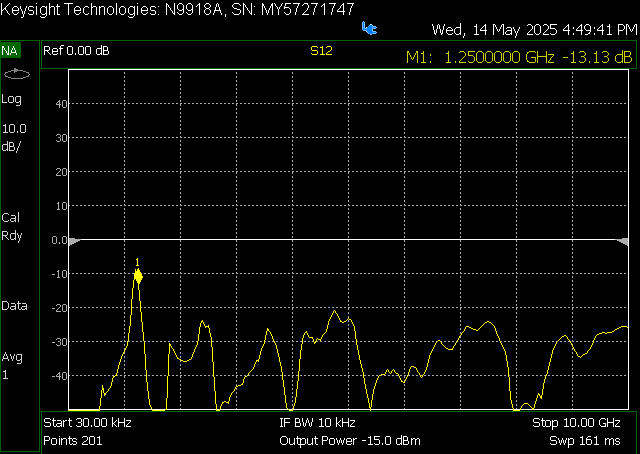
\includegraphics[width=\linewidth]{Pictures/S12neuCooleGrupp.png}
            \caption*{S21}
        \end{minipage}
        \hfill
        \begin{minipage}{0.45\textwidth}
            \centering
            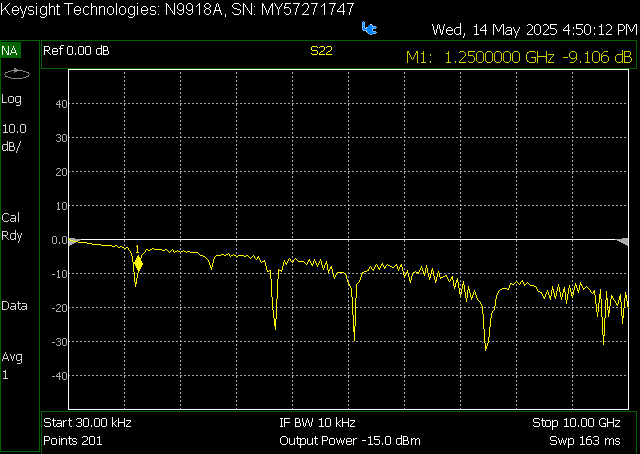
\includegraphics[width=\linewidth]{Pictures/S22neuCooleGruppe.png}
            \caption*{S22}
        \end{minipage}    
        \caption{Gemessene S-Parameter des Coupled-Line-Filters.}
        \label{fig:fieldfox_s_parameter}
    \end{figure}
    Diese Diagramme zeigen die entsprechenden Dämpfungen in Abhängigkeit von der Frequenz. Das Spektrum beginnt bei 30~kHz und endet bei 10~GHz, was unten im jeweiligen Diagramm abzulesen ist. 
    
    Man erkennt im Diagramm S12 bzw. S21 einen kleinen Peak bei 1,25~GHz, was darauf hindeutet, dass der Filter bei dieser Frequenz einen höheren Dämpfung aufweist. Die Dämpfung ist in diesem Fall bei S12 und S21 am geringsten und beträgt -13,13~dB, was darauf hinweist, dass der Filter in der Lage ist, Signale bei 1,25~GHz gut zu übertragen.
    Dies ist genau die Frequenz, bei der der bereitgestellte Transmitter funktioniert.
\section{Anschluss an den Transmitter und Messung im SA-Modus}
    Als Nächstes wird der Filter vom FieldFox abgekoppelt und mit dem Transmitter mittels einer SMA-Verbindung zur Erzeugung eines Signals verbunden. Am Transmitter wird hierbei eine Spannung $V_\mathrm{CO}$ von 5~V angelegt.
    Der Transmitter erzeugt ein Signal bei 1,20~GHz, welches durch den Filter geleitet wird. Der FieldFox wird in den Spectrum-Analyzer-Modus versetzt, um die Leistung des Signals zu messen. 
    Somit ist die Messung bei 1,20~GHz von Relevanz, da dies die Frequenz ist, bei der der Filter am besten funktioniert.

    \subsection{Leistungsmessung des Transmitters ohne Filter}
    Folgendes Leistungsspektrum am Transmitter ohne Filter wird gemessen:
    \begin{figure}[H]
        \centering
        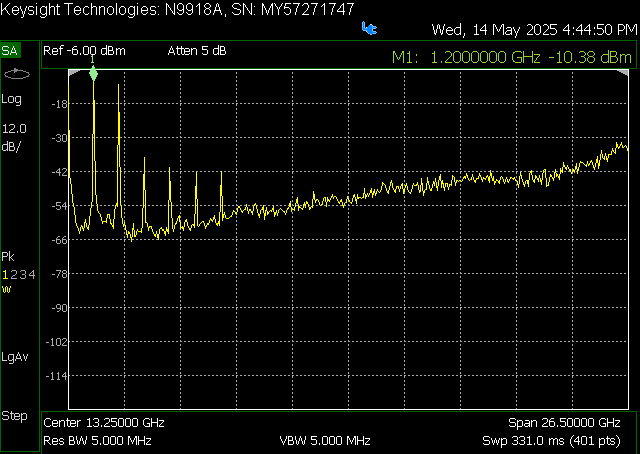
\includegraphics[width=0.6\linewidth]{Pictures/SA-TranceiverohnegutFIlterPeakCooleGrupp.png}
        \caption{Leistungsspektrum des Transmitters ohne Filter.}
        \label{fig:transmitter_spectrum_without_filter}
    \end{figure}
    Dieses zeigt einen Peak bei 1,20~GHz, was die Frequenz des Signals ist, das der Transmitter erzeugt. Die Leistung des Signals beträgt etwa -10~dBm.
    \subsection{Leistungsmessung des Transmitters mit Filter}
    Im Anschluss wird der Filter zwischen dem Transmitter und dem FieldFox geschaltet, um die Leistung des Signals zu messen, das durch den Filter geleitet wird.
    Folgendes Leistungsspektrum wird gemessen:
    \begin{figure}[H]
        \centering
        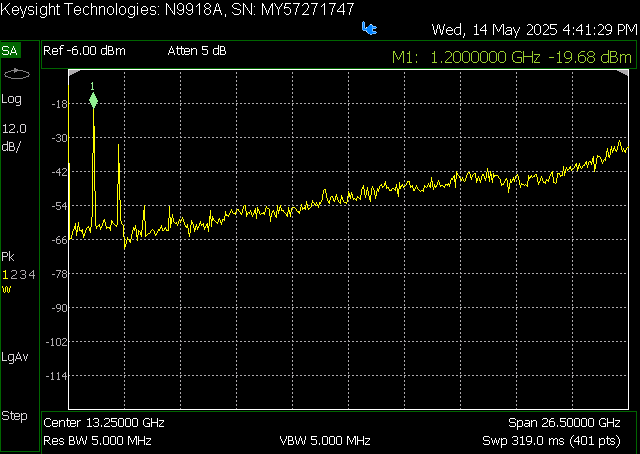
\includegraphics[width=0.6\linewidth]{Pictures/SA-TranceiverMitFIlterPeakCooleGruppe.png}
        \caption{Leistungsspektrum des Transmitters mit Filter.}
        \label{fig:transmitter_spectrum_with_filter}
    \end{figure}
    Es ist wieder ein Peak bei 1,20~GHz zu erkennen, jedoch ist die Leistung des Signals nun bei etwa -19~dBm. 
\section{Vergleich des gefilterten und ungefilterten Spektrums}
Als Fazit lässt sich schließen, dass der Filter die Leistung des Signals bei 1,20~GHz um etwa 9~dB reduziert hat. Trotzdem ist der Filter in der Lage, andere Frequenzen zu dämpfen, was ein Bandpassverhalten ist. 
Der Filter hat somit die Aufgabe, unerwünschte Frequenzen zu dämpfen und das Signal bei 1,20~GHz zu erhalten. 
Die Dämpfung des Signals bei 1,20~GHz ist zwar nicht ideal, aber der Filter erfüllt seine Aufgabe, indem er andere Frequenzen dämpft und das Signal bei 1,20~GHz erhält.